\documentclass[11pt,a4paper]{article}

\usepackage[utf8]{inputenc}
\usepackage[spanish]{babel}
\usepackage{amsmath}
\usepackage{float}
\usepackage{amsfonts}
\usepackage{amssymb}
\usepackage{makeidx}
\usepackage{graphicx}
\usepackage{lmodern}
\usepackage{kpfonts}
\usepackage{wrapfig}
\usepackage{caption}
\usepackage{subcaption}
\usepackage{booktabs}
\usepackage[nottoc,numbib]{tocbibind} %agrega la bibliografia al índice.
\usepackage[font={small,it}]{caption}
%\usepackage{fourier}
\usepackage[left=2cm,right=2cm,top=2cm,bottom=2cm,headheight=13.6pt]{geometry}
\usepackage{fancyhdr}
\usepackage{multirow}
\pagestyle{fancy}


%Para los gráficos en general, con las tablas...¡Ja!, arreglate.
%\begin{figure}[h!]
%\centering
%\includegraphics[width=0.7\textwidth]{} %nombre de la imagen, incluirla en el mismo directorio que este archivo.
%\caption*{} %rótulo, el asterico elimina la numeración automática. 
%\label{fig:} % para luego referirse con \ref{fig:}
%\end{figure}


\begin{document}


%%%%%%%%%%%%%%%%%%%%%%%%%%%%%%%%%%%%%%%%%%%%%%%%%%%%%%%%%%%%%%%%%%%%%%%%%%%%%%%%%%%%%%%%%%%%%%%%%%%%%%%%%%%%%%%%%%%%%%%%%%%%%%%%%
% 	TÍTULO
%%%%%%%%%%%%%%%%%%%%%%%%%%%%%%%%%%%%%%%%%%%%%%%%%%%%%%%%%%%%%%%%%%%%%%%%%%%%%%%%%%%%%%%%%%%%%%%%%%%%%%%%%%%%%%%%%%%%%%%%%%%%%%%%%

%%%%%%%%%%%%%%%%%%%%%%%%%%%%%%%%%%%%%%%%%
% University Assignment Title Page 
% LaTeX Template
% Version 1.0 (27/12/12)
%
% This template has been downloaded from:
% http://www.LaTeXTemplates.com
%
% Original author:
% WikiBooks (http://en.wikibooks.org/wiki/LaTeX/Title_Creation)
%
% License:
% CC BY-NC-SA 3.0 (http://creativecommons.org/licenses/by-nc-sa/3.0/)
% 
% Instructions for using this template:
% This title page is capable of being compiled as is. This is not useful for 
% including it in another document. To do this, you have two options: 
%
% 1) Copy/paste everything between \begin{document} and \end{document} 
% starting at \begin{titlepage} and paste this into another LaTeX file where you 
% want your title page.
% OR
% 2) Remove everything outside the \begin{titlepage} and \end{titlepage} and 
% move this file to the same directory as the LaTeX file you wish to add it to. 
% Then add \input{./title_page_1.tex} to your LaTeX file where you want your
% title page.
%
%%%%%%%%%%%%%%%%%%%%%%%%%%%%%%%%%%%%%%%%%

%----------------------------------------------------------------------------------------
%	PACKAGES AND OTHER DOCUMENT CONFIGURATIONS
%----------------------------------------------------------------------------------------

%\documentclass[12pt]{article}
%\usepackage[utf8]{inputenc}
%\usepackage[spanish]{babel}
%\begin{document}

\begin{titlepage}

\newcommand{\HRule}{\rule{\linewidth}{0.5mm}} % Defines a new command for the horizontal lines, change thickness here

\center % Center everything on the page
 
%----------------------------------------------------------------------------------------
%	HEADING SECTIONS
%----------------------------------------------------------------------------------------

\textsc{\Huge Universidad de Buenos Aires}\\[0.5cm]
\textsc{\LARGE Facultad de Ciencias Exactas y Naturales}\\[0.5cm] % Name of your university/college
\textsc{\Large Departamento de Física}\\[0.25cm] % Major heading such as course name

\begin{figure}[h]
  \centering
  
\includegraphics[scale=0.15]{Logo_DF}
  \\[0.5cm]
\end{figure}

\textsc{\large Laboratorio 3}\\[0.25cm] % Minor heading such as course title

%----------------------------------------------------------------------------------------
%	TITLE SECTION
%----------------------------------------------------------------------------------------

\HRule \\[0.4cm]
{ \huge \bfseries Transitorio y tiempo caracteristico de circuitos}\\[0.2cm] % Title of your document
\HRule \\[1cm]
 
%----------------------------------------------------------------------------------------
%	AUTHOR SECTION
%----------------------------------------------------------------------------------------

\begin{minipage}{0.4\textwidth}
\begin{center} \large
\emph{Autores:}\\
\textsc{Andreu}, Gonzalo\\ % Your name
\textsc{Malpartida}, Bryan\\ % Your name
\textsc{Pugliese}, Facundo\\ % Your name


\end{center}
\end{minipage}
~ \\[1.25cm]
%\begin{minipage}{0.4\textwidth}
%\begin{flushright} \large
%\emph{Supervisor:} \\
%Dr. James \textsc{Smith} % Supervisor's Name
%\end{flushright}
%\end{minipage}\\[4cm]

% If you don't want a supervisor, uncomment the two lines below and remove the section above
%\Large \emph{Author:}\\
%John \textsc{Smith}\\[3cm] % Your name

%----------------------------------------------------------------------------------------
%	DATE SECTION
%----------------------------------------------------------------------------------------

%\vspace{\fill}


{\large 17 de Febrero de 2016}\\[1.75cm] % Date, change the \today to a set date if you want to be precise

%----------------------------------------------------------------------------------------
%	SUMMARY SECTION: No más de 15 renglones, no te zarpes
%----------------------------------------------------------------------------------------

\begin{center}
\large{\textbf{Resumen}}

\small{El objetivo del siguiente trabajo fue caracterizar circuitos RC, RL y RCL. 

Para los dos primeros casos, los circuitos RC y RL, se buscó determinar el tiempos característico de cada uno variando los parámetros de cada sistema. Ademas de poder observar los fenómenos particulares en estos sistemas, como la carga y descarga del capacitor y la disminución de la corriente debido a la inductancia, utilizando una fuente de alimentación que emitía señales cuadradas y osciloscopio como instrumento de medición.

Por otro lado, el estudio del circuito RCL se centró en la observación de los comportamientos que tiene el mismo para distintos parámetros del sistema. Para ellos se obtenían teóricamente los valores necesarios de cada parámetro para luego $settear$ los elementos del circuito y comprobar que la evolución del sistema cumpliese el modelo teórico. Dichas observaciones se obtuvieron nuevamente utilizando una fuente de señal cuadrada y un osciloscopio.

Finalmente, el método resulto eficiente a la hora de comprobar las ecuaciones referidas al circuito RC y, en menor medida, al circuito RL. En el caso del circuito RCL, pudieron analizarse los casos extremos de comportamiento, pero no el comportamiento borde debido a lo fino del mismo.} % ACA VA EL RESUMEN

\end{center}


%----------------------------------------------------------------------------------------
%	LOGO SECTION
%----------------------------------------------------------------------------------------

%\includegraphics{Logo}\\[1cm] % Include a department/university logo - this will require the graphicx package
 
%----------------------------------------------------------------------------------------

\vfill % Fill the rest of the page with whitespace

\end{titlepage}
%\end{document} %incluir en el mismo directorio que este archivo. Equivalente a un copiar-pegar, nada de andar diciendo \begin{document} en la portada. Dejar el nombre de Caratula a la caratula.

%%%%%%%%%%%%%%%%%%%%%%%%%%%%%%%%%%%%%%%%%%%%%%%%%%%%%%%%%%%%%%%%%%%%%%%%%%%%%%%%%%%%%%%%%%%%%%%%%%%%%%%%%%%%%%%%%%%%%%%%%%%%%%%%%
% 	ENCABEZADO Y PIE DE PÁGINA.
%%%%%%%%%%%%%%%%%%%%%%%%%%%%%%%%%%%%%%%%%%%%%%%%%%%%%%%%%%%%%%%%%%%%%%%%%%%%%%%%%%%%%%%%%%%%%%%%%%%%%%%%%%%%%%%%%%%%%%%%%%%%%%%%%

\lhead{}
\chead{}
\rhead{Laboratorio 3}
\lfoot{}
\cfoot{}
\rfoot{\thepage}
\renewcommand{\headrulewidth}{1pt}
\renewcommand{\footrulewidth}{1pt}


%%%%%%%%%%%%%%%%%%%%%%%%%%%%%%%%%%%%%%%%%%%%%%%%%%%%%%%%%%%%%%%%%%%%%%%%%%%%%%%%%%%%%%%%%%%%%%%%%%%%%%%%%%%%%%%%%%%%%%%%%%%%%%%
% Página en blanco. Cita, agradecimiento, dedicación, lo que sea pero que sea algo.
%%%%%%%%%%%%%%%%%%%%%%%%%%%%%%%%%%%%%%%%%%%%%%%%%%%%%%%%%%%%%%%%%%%%%%%%%%%%%%%%%%%%%%%%%%%%%%%%%%%%%%%%%%%%%%%%%%%%%%%%%%%%%%%


%%%%%%%%%%%%%%%%%%%%%%%%%%%%%%%%%%%%%%%%%%%%%%%%%%%%%%%%%%%%%%%%%%%%%%%%%%%%%%%%%%%%%%%%%%%%%%%%%%%%%%%%%%%%%%%%%%%%%%%%%%%%%%%%%
% 	ÍNDICE
%%%%%%%%%%%%%%%%%%%%%%%%%%%%%%%%%%%%%%%%%%%%%%%%%%%%%%%%%%%%%%%%%%%%%%%%%%%%%%%%%%%%%%%%%%%%%%%%%%%%%%%%%%%%%%%%%%%%%%%%%%%%%%%%%

%\tableofcontents %compilar dos o tres veces para verlo bien. ¡Todo un índice en unas cuantas letras!
%\newpage

%%%%%%%%%%%%%%%%%%%%%%%%%%%%%%%%%%%%%%%%%%%%%%%%%%%%%%%%%%%%%%%%%%%%%%%%%%%%%%%%%%%%%%%%%%%%%%%%%%%%%%%%%%%%%%%%%%%%%%%%%%%%%%%
% 1. RESUMEN
%%%%%%%%%%%%%%%%%%%%%%%%%%%%%%%%%%%%%%%%%%%%%%%%%%%%%%%%%%%%%%%%%%%%%%%%%%%%%%%%%%%%%%%%%%%%%%%%%%%%%%%%%%%%%%%%%%%%%%%%%%%%%%%

%\section{Resumen}
%\label{sec:resumen}



%%%%%%%%%%%%%%%%%%%%%%%%%%%%%%%%%%%%%%%%%%%%%%%%%%%%%%%%%%%%%%%%%%%%%%%%%%%%%%%%%%%%%%%%%%%%%%%%%%%%%%%%%%%%%%%%%%%%%%%%%%%%%%%
% 2. INTRODUCCIÓN: ecuaciones aquí, luego se las cita.
%%%%%%%%%%%%%%%%%%%%%%%%%%%%%%%%%%%%%%%%%%%%%%%%%%%%%%%%%%%%%%%%%%%%%%%%%%%%%%%%%%%%%%%%%%%%%%%%%%%%%%%%%%%%%%%%%%%%%%%%%%%%%%%

\section{Introducción}\label{sec:intro}

\subsection{Campos magnéticos estacionarios}

El primer campo estacionario que se estudiará será el campo magnético terrestre. Debido al núcleo de hierro en el interior del planeta se genera un campo magnético $\vec{B}$ como se ve en la \textbf{Figura \ref{subfig:Campo_B}}.

\begin{figure}[h]

\begin{subfigure}{0.5\textwidth}
\centering
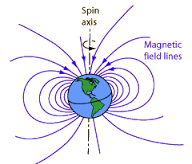
\includegraphics[scale=.8]{Campo.png}
	\subcaption{Campo magnético terrestre}
	\label{subfig:Campo_B}
\end{subfigure}
\begin{subfigure}{0.5\textwidth}
\centering
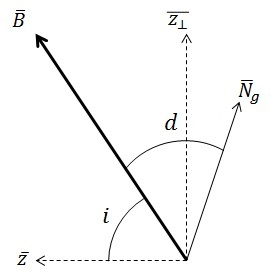
\includegraphics[scale=.65]{angulos_campo.jpg}
	\subcaption{Se definen $i$ es la inclinación y $d$ la declinación del campo magnético terrestre.}
	\label{subfig:Angulos}
\end{subfigure}
\caption{Relación angular entra el campo magnético y el eje de rotación.}
\end{figure}

Siendo que el eje de rotación y del campo magnético están inclinados uno respecto del otro, se pueden definir la \textit{inclinación} $i$ como el ángulo que forma $\vec{B}$ y el vector $\vec{z}$ que va al centro del planeta; y la \textit{declinación} $d$ como el ángulo entre $\vec{B}$ y el vector del norte geográfico $\vec{N_g}$ (ver \textbf{ Figura \ref{subfig:Angulos}}). Es claro que estos ángulos depende de la posición geográfica de donde se lo mida.

\bigskip
El siguiente campo estacionario es el generado por una bobina. Si se considera una bobina de largo $L$, radio $r$ y con $N$ cantidad de vueltas, como se ve en la \textbf{Figura \ref{fig:bobina_intro}},

\begin{figure}[h]

\centering
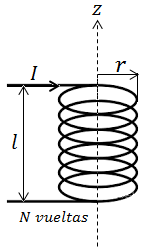
\includegraphics[scale=1]{bobina.png}
	\caption{Bobina de largo $l$, radio $r$ y con $N$ cantidad de vueltas por el cual circula una corriente $I$.}
	\label{fig:bobina_intro}
\end{figure}

al hacer circular una corriente $I$ se genere un campo magnético. Tomando el origen $0$ en el punto medio de la bobina que pasa por el eje de simetría $z$, de modo que ambos extremos se encuentre a distancia $\frac{l}{2}$ de dicho origen; el valor del campo sobre los puntos $z=0$ y $z=\pm \frac{l}{2}$ serán:

\begin{equation}{\label{valores_B}}
\begin{split}
B(0,0, \pm \frac{l}{2})= \frac{\mu I N}{2\sqrt{R^2+l^2}}\\
B(0,0,0)= \frac{\mu I N}{2\sqrt{R^2+(\frac{l}{2})^2}}
\end{split}
\end{equation}

Donde $\mu$ es la permeabilidad magnética del medio. Ademas, la inductancia $L$ de la bobina es

\begin{equation}
L=\frac{2\pi\mu N^2 r}{l}
\end{equation}

\subsection{Transformadores}
Un transformador es un sistema en el cual un circuito activo o \textit{primario}, con inductancia $L_1$, transmite energía a un circuito pasivo o \textit{secundario} con inductancia $L_2$. Este fenómeno se debe a la inductancia mutua $M$ entre ambos circuitos armando el sistema como se ve en la \textbf{Figura \ref{fig:transformador}}.

\begin{figure}[h]
\centering
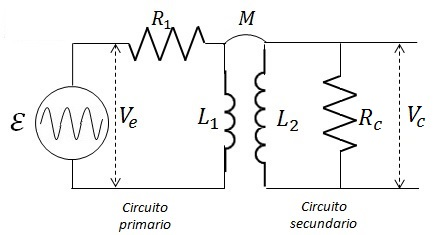
\includegraphics[scale=.8]{transformador.jpg}
\caption{Transformador}
\label{fig:transformador}	
\end{figure}

Si la fuente $\varepsilon$ varia en el tiempo de la forma $\varepsilon (t) = E_0 sin (\omega t)$, al resolver el circuito utilizando las leyes de Kirchoff, la transferencia tiene una expresión compleja:

\begin{equation}
\frac{V_c}{V_e}= \frac{i\omega M R_c}{(R_1 + i\omega L_1)(R_c + i\omega L_2)+ (\omega M)^2}
\label{transf_1}
\end{equation}

Bajo la condición $R_1 \ll \omega L_1$, la solución anterior se puede simplificar en:

\begin{equation}
\frac{V_c}{V_e}=\frac{MR_c}{L_1R_c-i\omega L_1L_2(1-k^2)}
\label{transf_2}
\end{equation}

En este caso la inductancia mutua se puede expresar como $M^2=K^2L_1L_2$ siendo $\vert k\vert\leq1$. Solo en el caso ideal $\vert k\vert = 1$, por lo que si entre las bobinas se coloca un núcleo de un material ferromagnético, por ejemplo hierro, se tendrá $\vert k\vert \simeq 1$; de modo que, en la aproximación al caso ideal, la transferencia del transformador es:

\begin{equation}
\frac{V_c}{V_e}= \sqrt{\frac{L_1}{L_2}}
\label{trans_3}
\end{equation}



%%%%%%%%%%%%%%%%%%%%%%%%%%%%%%%%%%%%%%%%%%%%%%%%%%%%%%%%%%%%%%%%%%%%%%%%%%%%%%%%%%%%%%%%%%%%%%%%%%%%%%%%%%%%%%%%%%%%%%%%%%%%%%%
% 3. DISPOSITIVO EXPERIMENTAL: armado del modelo, como se midio, consideraciones a la hora de medir.
%%%%%%%%%%%%%%%%%%%%%%%%%%%%%%%%%%%%%%%%%%%%%%%%%%%%%%%%%%%%%%%%%%%%%%%%%%%%%%%%%%%%%%%%%%%%%%%%%%%%%%%%%%%%%%%%%%%%%%%%%%%%%%%

\section{Desarrollo experimental}

Durante esta experiencia se utilizó un generador de funciones de generar diferencias de potencial $V(t)$ a frecuencias con un error relativo del $0,01\%$ en un rango entre $1\mu Hz$ y $5MHz$. El voltaje pico-pico tiene un error relativo del $1\%$ para el rango de voltaje utilizado ($2V-20V$). Además, se utilizó una resistencia variable por décadas en el intervalo $1\Omega-11110\Omega$. Usando un multimetro digital se midieron los valores utilizados en esta resistencia junto con su precisión que era de la forma $\pm(1\%+2d)$ en el rango utilizado (mayor a $100\Omega$). El multimetro permitía también medir diferencias de potencial con una precisión de la forma $(1d+0,5\%)$.

Para generar una diferencia de potencial constante se utilizó una fuente de alimentación programable con una precisión de $\pm (0.5\% + 0.02)V$ en un rango de voltaje de salida de $0 \thicksim 32 V$. Esta fuente también era capaz de generar corrientes constantes $I$. Se utilizó además un osciloscopio digital que en sus dos canales de entrada era capaz de medir diferencias de potencial entre sus dos terminales en un rango de 2mV a 5V con un error relativo del $3\%$. A la hora de medir voltaje, fue necesario asegurarse que el cable a tierra del osciloscopio estuvera conectado al cable a tierra el generador de funciones. 

Finalmente, se utilizó un sensor Hall capaz de medir el módulo de campos magnéticos $B$ en una dirección particular, expresándolos como una diferencia de potencial $V$. La relación entre $B$ y $V$ está dada por $B = mV+offset$ donde $m$ es una característica del instrumento definida por su ganancia $G$ y su sensibilidad $S$ según $m = S^{-1}$. La ganancia $G$ puede ser x1, x10 o x200 y define una sensibilidad $S_{x1} = (3,06 \pm 0,15)\frac{mV}{G}$,  $S_{x10} = (30,6 \pm 1,2)\frac{mV}{G}$ y $S_{x200} = (612 \pm 24)\frac{mV}{G}$. Por lo tanto, las pendientes resultan $m_{x1} = (327 \pm 5)\frac{G}{V}$, $m_{x10} = (32,7 \pm 1,3)\frac{G}{V}$ y $m_{x200} = (1,63 \pm 0,06)\frac{G}{V}$. La caracterización del $offset$ se cubre a continuación.

\subsection{Caracterización del Sensor Hall y medición del campo magnético terrestre}

Como se dijo más arriba, a la hora de calcuar la intensidad de un campo megnético $B$, es necesario caracterizar el parámetro $offset$. Una forma de obtenerlo es midiendo el campo magnético $B^{+} = m.V^{+}+offset$ en una dirección $\widehat{u}$ y luego medir en la dirección opuesta $-\widehat{u}$el campo $B^{-} = m.V^{-}+offset=-B^{+}$. De esta forma es posible obtener $offset = \frac{m}{2}(V^{+}+V^{-})$. Esto se hizo efectivamente midiendo el campo magnético terrestre en una dirección $\widehat{u}$ aleatoria. Se midió en esa misma dirección con las 3 escalas posibles del sensor hall. Cabe aclarar que la diferencia de potencial generada por el Sensor Hall fue medida a través de un voltímetro en su función de amperímetro.

Una vez caracterizado el $offset$, el sensor fue utilizado para medir la dirección y magnitud del campo magnético terrestre en el laboratorio. Se lo montó sobre un soporte con una nuez y se lo fue rotando en el plano perpendicular al tripode hasta encontrar un máximo. Luego se rotó el sensor en su propio plano hasta encontrar nuevamente un máximo. Este último valor fue el que se asignó como la magnitud del campo y con los dos angulos relativos se caracterizó su dirección (ver \textbf{Figura \ref{fig:terrestre}}).


\begin{figure}[h!]
\centering
   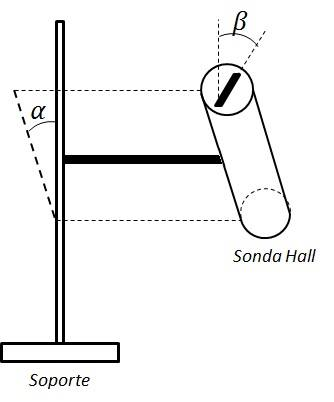
\includegraphics[width=0.7\textwidth]{Terrestre}
   \caption{Esquema de la bobina utilizada con sus parámetros definidos: $r = (46,7 \pm 0,1)mm$, $l = (255 \pm 5)mm$ y $d = (33 \pm 5)mm$}  
   \label{fig:terrestre}
\end{figure}

\subsection{Caracterización de una bobina}

Posteriormente, se tomó una bobina de radio $r = (46,7 \pm 0,1)mm$ separada en dos secciones idénticas, cada una con un embobinado de $N$ vueltas desconocido (ver \textbf{Figura \ref{fig:bobina}}). La longitud del embobinado fue $l = (255 \pm 5)mm$ mientras que la longitud de la sección superior era $l_1 = (111,2 \pm 0,1)mm = l_2$, por lo que resultaba $d = (33 \pm 5)mm$. Estas magnitudes fueron medidas utilizando un calibre digital y una regla, lo cual puede notarse en la diferencia de errores. 

\begin{figure}[h!]
\centering
   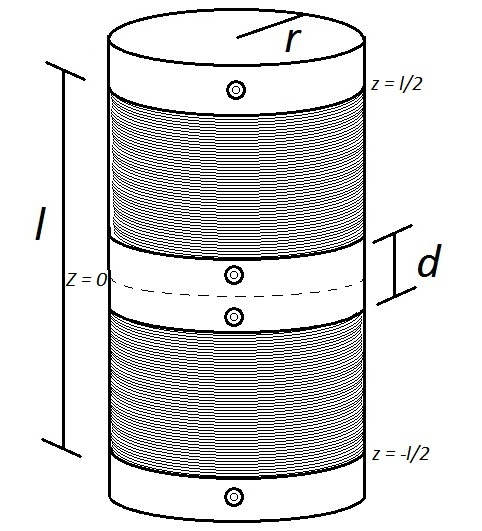
\includegraphics[width=0.7\textwidth]{Bobina}
   \caption{Esquema de la bobina utilizada con sus parámetros definidos: $r = (46,7 \pm 0,1)mm$, $l = (255 \pm 5)mm$ y $d = (33 \pm 5)mm$}  
   \label{fig:bobina}
\end{figure}

Con el objetivo de estimar $N$, se probaron diversos métodos. El primero consistió en hacer circular una corriente conocida $I$ a través de los circuitos de la \textbf{Figura \ref{fig:circ_bob}}. Despreciando la inducción de la bobina (en ambos formatos), las corrientes $I$ eran constantes. En ambas configuraciones, se ubicó el Sensor Hall en el extremo superior de la bobina ($z = \frac{l}{2}$) y se lo conectó a un voltímetro para poder medir las diferencias de potencial $V$ y de allí obtener $B$. Cabe aclarar que se buscó que el sensor estuviera ubicado sobre el eje vertical de la bobina, para lo cual se utilizó el calibre. Para complemental, se realizaron estas mediciones nuevamente para la bobina completa, pero con el sensor ubicado en $z = 0$ y aún centrado. 

\begin{figure}[h!]
   \begin{subfigure}{0.5\textwidth}
      \centering
      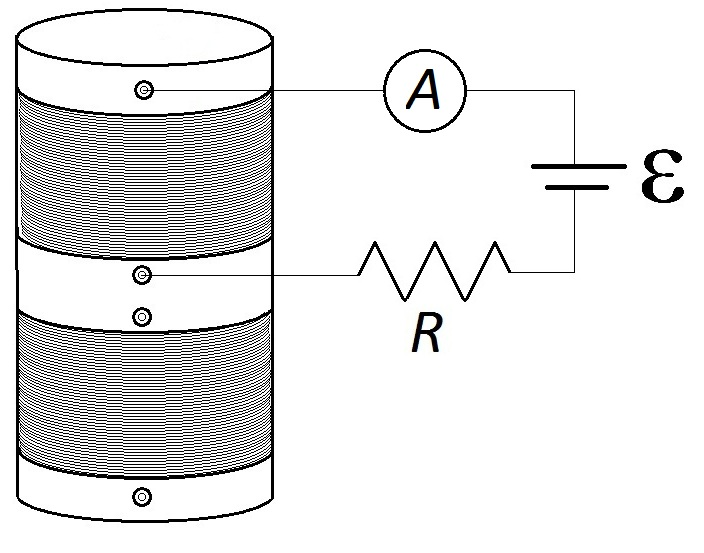
\includegraphics[width=0.7\textwidth]{Circuito_Bobina_corta}
      \caption{Circuito utilizando la mitad superior de la bobina, aquí resulta $l_1 = (111,2 \pm 0,1)mm$ y $r = (46,7 \pm 0,1)mm$}  
      \label{subfig:bob_corta}
   \end{subfigure}
   \begin{subfigure}{0.5\textwidth}
      \centering
      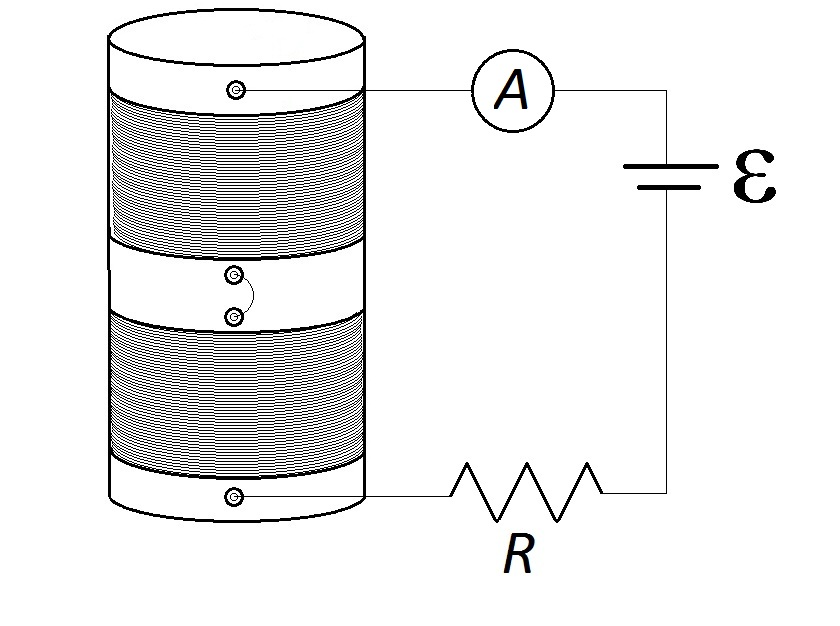
\includegraphics[width=0.7\textwidth]{Circuito_Bobina_larga}
      \caption{Circuito utilizando la bobina completa, aquí resulta $r = (46,7 \pm 0,1)mm$, $l = (255 \pm 5)mm$ y $d = (33 \pm 5)mm$ como antes}  
      \label{subfig:bob_larga}
   \end{subfigure}
   \caption{Circuitos sobre los que se hizo circular distintas corrientes constantes $I$ (despreciando la induccción) para obtener distintos campos magnéticos $B$. El sensor magnético es externo y se ubicó en la parte superior de la bobina.}
   \label{fig:circ_bob}
\end{figure}

Finalmente, para la configuración que solo utilizaba la parte superior, se ubicó el sensor a la altura $z = \frac{l}{2}$ y se calculó el campo magnético $B$ en función de la distancia $a$ al centro. Cabe aclarar que en todas los calculos de $B$ apareció una componente $B_{T}$ del campo magnético terrestre que no interfirió con las mediciones, dado que la relación \textbf{CAMPO DE BOBINA} solo agregaría una ordenada $B_T$.

Como segundo método, se midió la inductancia de ambas configuraciones (completa y mitad superior) con el objetivo de obtener $N$ a través de la ecuación \textbf{INDUCTANCIA DE BOBINA} y de los parámetros mencionados más arriba. Para esto se utilizó un medidor LCR cuya precisión a la hora de medir inductancias era del $(1,2\%+5d)$ para el rango en que se ubicaron las inductancias ($1999,9\mu H-19,999mH$).


\subsection{Caracterización de transformadores}

Para comenzar esta sección, se planteó montar un transformador de acople ideal. Para esto se usaron dos bobinas capaces de encajar una dentro de la otra como puede verse en la \textbf{Figura \ref{fig:transmont}}. Como la superposición no era perfecta dado que los radios eran distintos, se utilizó una barra de hierro en el interior de ambos para aumentar el flujo magnético. La bobina interior tenia una inductancia $L_1 = (78,4 \pm 0,8)\mu H$, una resistencia $R_{L_1}=(1,0 \pm 0,2)\Omega$ y un total de $N_1=235$ vueltas. La bobina externa tenía una inductancia $L_2 = (64,3 \pm 0,7)mH$, una resistencia $R_{L_2}=(79,0 \pm 0,6)\Omega$ y un total de $N_2=2920$ vueltas. Estas inductancias y resistencias fueron medidas con el medidor LCR y el multímetro, respectivamente.

\begin{figure}[h!]
\centering
   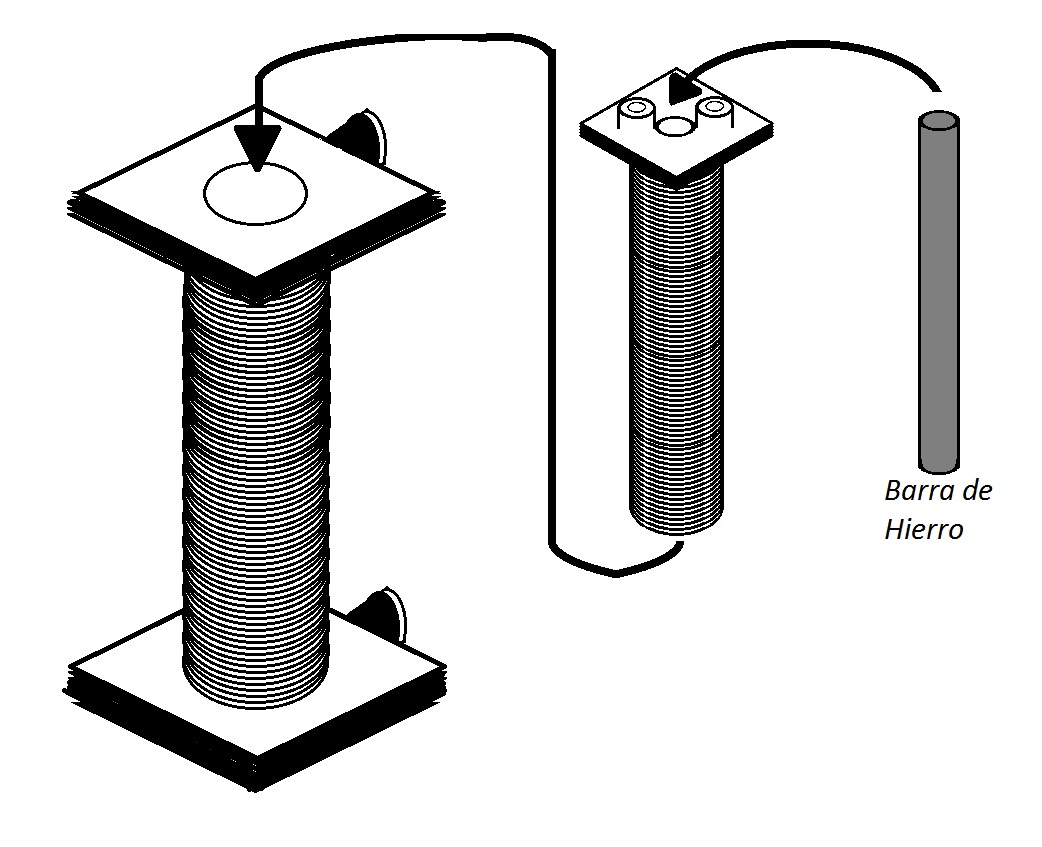
\includegraphics[width=0.7\textwidth]{Transformadores1}
   \caption{Montaje del transformador utilizando dos bobinas que encajaban una dentro de la otra. La barra de hierro se utilizó para mejorar el flujo magnético.}  
   \label{fig:transmont}
\end{figure}

Una vez montado el transformador, se armaron un par de circuitos que no tenian conexión (dado que las bobinas no estaban en contacto directo) como puede verse en la \textbf{Figura \ref{fig:trans1_circ}}. Para distintos voltajes de entrada $\varepsilon$ se registró la caída de potencial $V_R$ sobre la resistencia $R = (11,11 \pm 0,11)k\Omega$ con el osciloscopio. Conectando el generador al otro canal y usandolo como $trigger$ $externo$ pudo medirse el voltaje de entrada y el desfasaje entre $\varepsilon$ y $V_R$ con el objetivo de asegurarse que este último fuera constante. La frecuencia utilizada fue $f = (200000 \pm 20)Hz$, para asegurarse que se mantuviera la relación $R_1 = R_{L_1}+R_F << 2\pi fL_1$. Cabe destacar que como los circuitos no estaban conectados, no fue necesario conectar la tierra del osciloscopio a la tierra del generador de funciones. 


\begin{figure}[h!]
\centering
   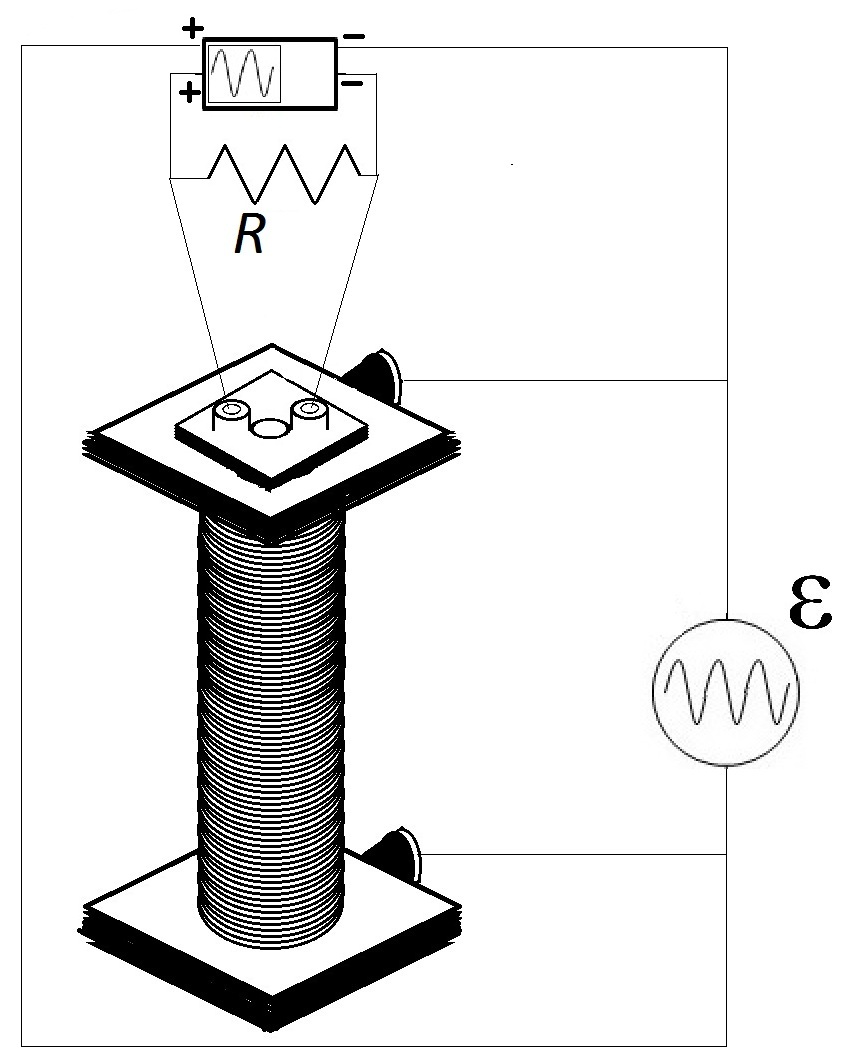
\includegraphics[width=0.7\textwidth]{Transformadores1_circuito}
   \caption{Par de circuitos acoplados a través del transformador. Se fue variando la amplitud de entrada $\varepsilon$ y registrando la diferencia de voltaje en la resistencia $R$.}  
   \label{fig:trans1_circ}
\end{figure}

Posteriormente, utilizando la misma configuración, se varió la frecuencia $f$ con el objetivo de relevar el desfasaje y la transmisión $\frac{V_R}{\varepsilon}$. Nuevamente, aunque se dejó la amplitud de la fuente constante, se la midió con el osciloscopio para cada frecuencia $f$.

De forma alternativa, se utilizaron dos configuraciones geométricas distintas con otras bobinas como muestra la \textbf{Figura \ref{fig:configs}} y se reemplazaron por el transformador de la \textbf{Figura \ref{fig:trans1_circ}}. La resistencia $R$ fue reemplazada por una nueva resistencia $R = (21,57 \pm 0,11)k\Omega$. Sin embargo, solo se varió la amplitud de entrada $\varepsilon$ y no se registró el desfasaje. Tampoco se varió la frecuencia, que fue fijada en cada configuración. En ambos casos, la bobina de menos vueltas fue la conectada al generador $\varepsilon$ y la de más vueltas a la resistencia $R$.

\begin{figure}[h!]
   \begin{subfigure}{0.5\textwidth}
      \centering
      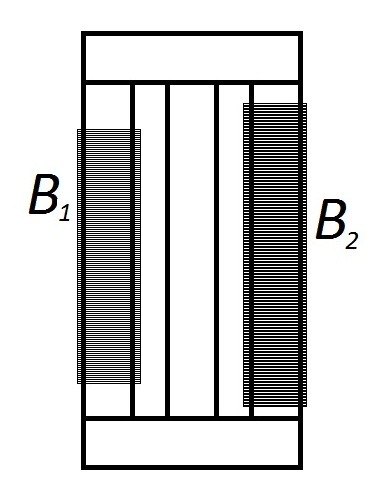
\includegraphics[width=0.7\textwidth]{configuracion1}
      \caption{Circuito utilizando la mitad superior de la bobina, aquí resulta $l_1 = (111,2 \pm 0,1)mm$ y $r = (46,7 \pm 0,1)mm$}  
      \label{subfig:con1}
   \end{subfigure}
   \begin{subfigure}{0.5\textwidth}
      \centering
      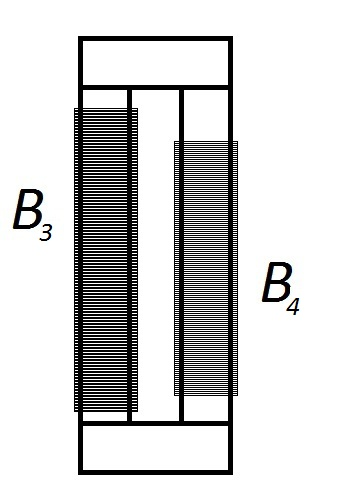
\includegraphics[width=0.7\textwidth]{configuracion2}
      \caption{Circuito utilizando la bobina completa, aquí resulta $r = (46,7 \pm 0,1)mm$, $l = (255 \pm 5)mm$ y $d = (33 \pm 5)mm$ como antes}  
      \label{subfig:con2}
   \end{subfigure}
   \caption{Distintas configuraciones de transformador cuyo soporte era de hierro. En ambos casos el circuito utilizado fue identico al de la \textbf{Figura \ref{fig:trans1_circ}}, aunque se modificó la resistencia $R$. El proceso de medición fue idéntico.}
   \label{fig:configs}
\end{figure}

Para la primer configuración del transformador, correspondiente a la \textbf{Figura \ref{subfig:con1}}, se utilizó como $B_1$ una bobina de 400 vueltas con $L_1 = (110 \pm 8)mH$ y $R_{L_1} = (5,8 \pm 0,2)\Omega$ y como $B_2$ una de 1600 vueltas con $L_2 = (1,54 \pm 0,01)H$ y $R_{L_2} = (194,0 \pm 0,3)\Omega$. Para esta configuración se utilizó una frecuencia $f = (150000 \pm 20)Hz$ para asegurarse de mantener la relación $R_1 = R_{L_1}+R_F << 2\pi fL_1$.

Para el transformador de la \textbf{Figura \ref{subfig:con2}} se utilizó una bobina $B_3$ de 200 vueltas con $L_3 = (10,63 \pm 0,08)mH$ y $R_{L_3} = (1,8 \pm 0,2)\Omega$ y una bobina $B_4$ de 800 vueltas con $L_4 = (169,6 \pm 1,2)mH$ y $R_{L_4} = (10,8 \pm 0,3)\Omega$. Nuevamente,  se utilizó una frecuencia $f = (300000 \pm 30)Hz$ para asegurarse de mantener la relación $R_3 = R_{L_3}+R_F << 2\pi fL_3$.



%%%%%%%%%%%%%%%%%%%%%%%%%%%%%%%%%%%%%%%%%%%%%%%%%%%%%%%%%%%%%%%%%%%%%%%%%%%%%%%%%%%%%%%%%%%%%%%%%%%%%%%%%%%%%%%%%%%%%%%%%%%%%%%%
% 4.DISCUSIÓN Y RESULTADOS: todo lo que se obtuvo y explicación. Graficos, tablas.
%%%%%%%%%%%%%%%%%%%%%%%%%%%%%%%%%%%%%%%%%%%%%%%%%%%%%%%%%%%%%%%%%%%%%%%%%%%%%%%%%%%%%%%%%%%%%%%%%%%%%%%%%%%%%%%%%%%%%%%%%%%%%%%%

\section{Resultados}
\label{sec:discusion}





%%%%%%%%%%%%%%%%%%%%%%%%%%%%%%%%%%%%%%%%%%%%%%%%%%%%%%%%%%%%%%%%%%%%%%%%%%%%%%%%%%%%%%%%%%%%%%%%%%%%%%%%%%%%%%%%%%%%%%%%%%%%%%%%
%	CONCLUSIONES
%%%%%%%%%%%%%%%%%%%%%%%%%%%%%%%%%%%%%%%%%%%%%%%%%%%%%%%%%%%%%%%%%%%%%%%%%%%%%%%%%%%%%%%%%%%%%%%%%%%%%%%%%%%%%%%%%%%%%%%%%%%%%%%%

\section{Conclusiones}
\label{sec:conclusiones}






%%%%%%%%%%%%%%%%%%%%%%%%%%%%%%%%%%%%%%%%%%%%%%%%%%%%%%%%%%%%%%%%%%%%%%%%%%%%%%%%%%%%%%%%%%%%%%%%%%%%%%%%%%%%%%%%%%%%%%%%%%%%%%%%%
%	APÉNDICE: esas cosas extras que simplemente no tuvieron lo suficiente como para ganarse una sección propia.
%%%%%%%%%%%%%%%%%%%%%%%%%%%%%%%%%%%%%%%%%%%%%%%%%%%%%%%%%%%%%%%%%%%%%%%%%%%%%%%%%%%%%%%%%%%%%%%%%%%%%%%%%%%%%%%%%%%%%%%%%%%%%%%%%



%%%%%%%%%%%%%%%%%%%%%%%%%%%%%%%%%%%%%%%%%%%%%%%%%%%%%%%%%%%%%%%%%%%%%%%%%%%%%%%%%%%%%%%%%%%%%%%%%%%%%%%%%%%%%%%%%%%%%%%%%%%%%%%%%
%	REFERENCIAS: libros, libros, libros.
%%%%%%%%%%%%%%%%%%%%%%%%%%%%%%%%%%%%%%%%%%%%%%%%%%%%%%%%%%%%%%%%%%%%%%%%%%%%%%%%%%%%%%%%%%%%%%%%%%%%%%%%%%%%%%%%%%%%%%%%%%%%%%%%%

%Ejemplo:
\begin{thebibliography}{1}
 \bibitem{Berkeley} Frank S. Crawford, \textit{Berkeley physics course 3: Ondas}, 1994, Editorial Reverte S.A.
\end{thebibliography}
%Para citar: blablabla \cite{Baird}
 
\end{document}





